\Aufgabe[e]{Dimensionierung eines Zugstabes}{
Die Querschnittsfläche eines Zugstabes soll dimensioniert werden.
Diese soll als positionsabhängige Funktion $A(x)$ bestimmt werden, siehe Abbildung.

Der Zugstab ist am oberen Ende fixiert und am unteren Ende mit einer konstanten Kraft $F_0\, [N]$ belastet.

Wie muss die Querschnittsfläche $A, [m^2]$ in Abhängigkeit von der Koordinate $x, [m]$ gewählt werden, damit die Zugspannung $\sigma\, [Pa]$ an jeder Schnittstelle den gleichen Wert $\sigma_c\, [Pa]$ hat?

\begin{itemize}
\item $L=10\, [cm]$: Länge des Zugstabes,
\item $A_0=0.002\, [m^2]$ : Querschnittsfläche am unteren Ende,
\item $\rho = 7.85 \, [g/cm^3]$: Dichte des Zugstabes als Funktion der Position $x$,
\item $g=9.81\, [m/s^2]$: Gravitationsbeschleunigung, 
\item $F_0=15\, [N]$: Konstante Belastung. 
\end{itemize}
\medskip

\begin{center}
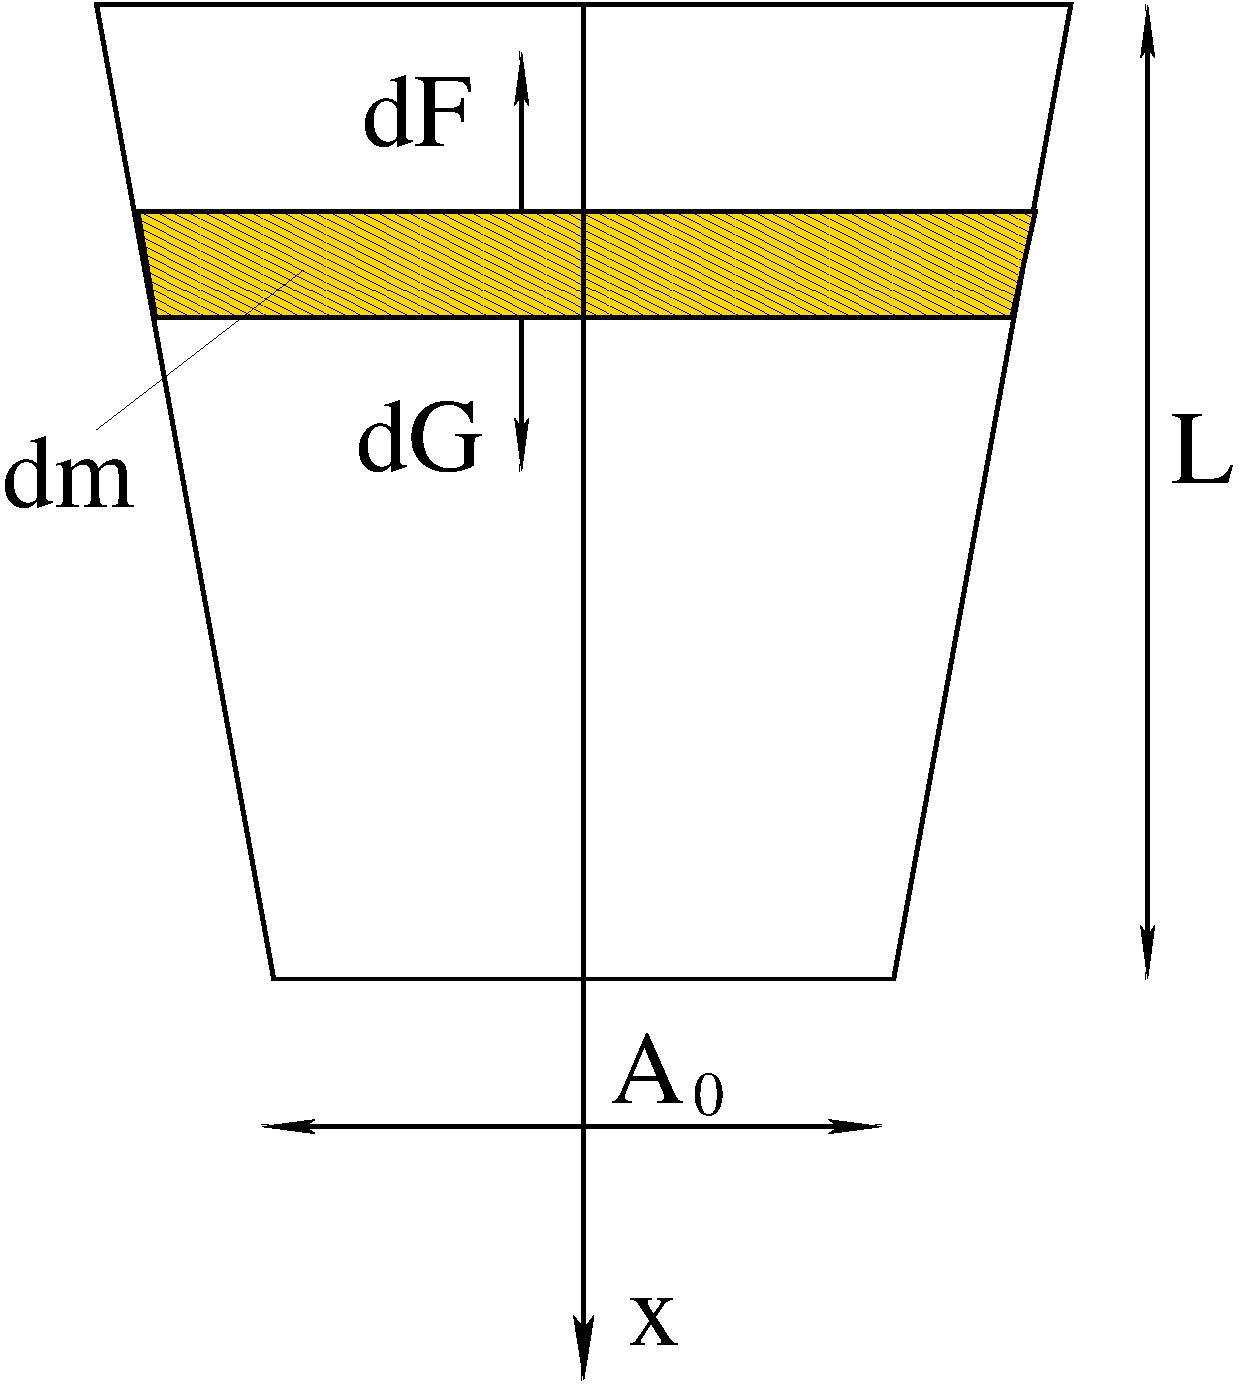
\includegraphics[width =0.18\textwidth]{../A/Wiederholung/Zugstab.pdf}
\end{center}

Lösungsansatz:\\

Auf das gelbe Massenelement in der Abbildung $\drm m = \rho \drm V = \rho A \drm x$ wirken die folgenden Kraftelemente ein
\begin{itemize}
\item Zugkraft: $\drm F =  \drm (\sigma(x) \drm A) = \sigma_c \drm A$, die über das Flächenelement $\drm A$ mit einer konstanten Zugspannung $\sigma_c$ wirkt,
\item Gewichtskraft: $\drm G = \rho g A \drm x$, die über das Volumenelement $\drm V=A\drm x$ wirkt.
\end{itemize}
%
Die Terme $\drm F$, $\drm A$ und $\drm x$ heißen Differentiale.
%
Das Massenelement befindet sich im Gleichgewicht, wenn die Zugkraft die Gewichtskraft in ihrer Wirkung ausgleicht. Somit gilt
\begin{align*}
\drm F + \drm G &= 0,\\
\end{align*}
oder
\begin{align*}
\sigma_c \drm A + \rho g A \drm x &= 0,
\end{align*}
%
Wir schreiben die Gleichung so um, dass die Variablen, $A$ und $x$, und ihre Differentiale getrennt sind
%
\begin{align*}
\frac{\drm A}{A} = -\frac{\rho g}{\sigma_c} \drm x.
\end{align*}
und integrieren beide Seiten.

\bigskip
\textbf{Hinweis}: Man beachte die Einheiten!
}
\Loesung{
Durch Integrieren erhält man
$$
\int \frac{1}{A}\drm A = -\frac{g}{\sigma_c} \rho\int 1 \, \drm x.
$$
Um die Fläche $A$ als Funktion von $x$ zu bestimmen muss man beide Seiten integrieren und anschließend die Integrationskonstante durch die Vorgabe $A(L)=A_0$ bestimmen. Die so bestimmte ortsabhängige Fläche erfüllt die Anforderung, dass die Spannung $\sigma$ konstant über $x$ ist.\\

Integriert man beide Seiten, erhält man
$$
\ln(A) + C_1 = -\frac{g}{\sigma_c} \rho x + C_2.
$$
Man kann beide Konstanten vereinigen und in mit Hilfe des Logarithmus darstellen als $\ln C = C_2-C_1$: 
$$
\ln(A) = -\frac{g}{\sigma_c}\, \rho x + \ln(C). 
$$


Man erhält
\begin{align*}
\ln(A)-\ln(C) &= -\frac{g}{\sigma_c} \rho x,\\
\ln(A/C) &= -\frac{g}{\sigma_c} \rho x,\\
A & = C\operatorname{e}^{-\frac{g}{\sigma_c} \rho x}.
\end{align*}
Um die Konstante $C$ zu bestimmen, setzt man $x=L$ und $A=A_0$ in die Formel
$$
A_0 = C \operatorname{e}^{-\frac{g}{\sigma_c} \rho L}
$$
und erhält
$$
C = A_0\operatorname{e}^{\frac{g}{\sigma_c} \rho L}.
$$
Die Querschnittsfläche ist dann
%
\begin{align*}
A &= A_0\operatorname{e}^{\frac{g}{\sigma_c} \rho L}\operatorname{e}^{-\frac{g}{\sigma_c} \rho x},\\
&= A_0\operatorname{e}^{\frac{g}{\sigma_c} \rho (L-x)}.
\end{align*}
Die Spannung $\sigma_c$ kann mit $F_0$ und $A_0$ bestimmt werden:
$$
\sigma_c = \frac{F_0}{A_0} = 7500 \text{ [$N$/$m^2$]}.
$$
Durch Umrechnen der Einheiten erhält man $L=0.1$ [$m$] und $\rho=7850$ [$kg$/$m^3$] und
$$
A(x) = 0.002 \operatorname{e}^{10.27\,(0.1-x)}.
$$
In dieser Gleichung wurden keine Einheiten angegeben, da zuvor alle Werte in SI-Einheiten umgerechnet werden. Somit liefert sie auch ein Ergebnis in SI-Einheiten (hier $m^2$). \\
Die Querschnittsfläche ist 0.002 $m^2$ (oder 20 $cm^2$) in $x=L$ und 0.0056 $m^2$ (oder 56 $cm^2$) in $x=0$.
}


\ErgebnisC{AufgZugstab}
{
$A(x) = A_0\operatorname{e}^{\frac{g}{\sigma_c} \rho (L-x)}.$

$A(x) = 0.002 \operatorname{e}^{10.27\,(0.1-x)}\quad \text{[$m^2$]}.$
}
